The Standard Model of particle physics is one of the most precisely tested
theories. It is a relatistivic quantum field theory using the Lagrange
formalism.

It provides a unified description of three of the four forces of nature: the
electromagnetic interaction, the weak interaction, and the strong
interaction. Gravitation not included.

Natural units $\hbar = c = 1$. Can be recovered by dimensional
analysis. Heaviside--Lorentz units?

Einstein summation convention: Sum over repeated indices.

Cross-sections in barn $\SI{1}{\barn} = 10^{-28}\,\si{\metre\squared}$

Cite what this description is based on: \cite{Halzen:1984mc,Thomson:2013zua}


\section{Particles and Interactions in the Standard Model}

The Standard Model, shown in~\Cref{fig:sm_particles}, consists of 12 elementary
spin-$\frac{1}{2}$ particles referred to as \emph{fermions} and their
anti-particles, and five types of particles with integer spin referred to as
\emph{bosons}. With the discovery of the Higgs boson in
2012~\cite{HIGG-2012-27,CMS-HIG-12-028}, experimental evidence for the existence
of all fermions and bosons predicted by the Standard Model is established.

\begin{figure}[htbp]
  \centering

  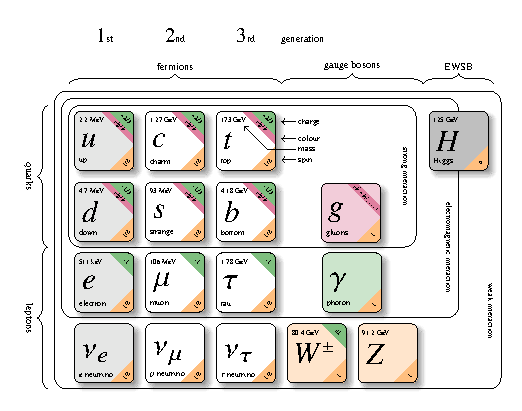
\includegraphics[width=\textwidth]{theory/sm}

  \caption{Particles of the SM. The diagram is adapted from Ref.~\cite{sm_tikz}
    with updated particle properties from Ref.~X. Antiparticles are not shown
    explicitly have additive quantum numbers of opposite sign but otherwise the
    same properties of the respective particle.}
  \label{fig:sm_particles}
\end{figure}


The elementary particles of the SM can be divided into three categories:
\begin{description}

\item[Fermions] predicted by the SM have spin-$\frac{1}{2}$. Consequently, they
  are massive\footnote{Neutrinos are considered as massless in the SM, however,
    the observation of neutrino
    oscillations~\cite{Super-Kamiokande:1998kpq,SNO:2002tuh} is experimental
    evidence for neutrinos having small but non-zero mass.} and adhere to the
  Pauli exclusion principle and are therefore considered to be \emph{matter}
  particles. For every fermions, a corresponding anti-particle exists that has
  the same properties but with opposite additive quantum numbers. The fermions
  of the SM are divided into \emph{quarks} that take part in the strong
  interaction and \emph{leptons} that do not. They are further divided into
  up-type quarks ($u$, $c$, $t$), down-type quarks ($d$, $s$, $b$), charged
  leptons ($e$, $\mu$, $\tau$), and neutrinos ($\nu_e$, $\nu_\mu$,
  $\nu_\tau$). The fermions of the SM come in three generations, the main
  difference between them being the mass of the fermions. All ordinary (stable)
  matter consists of fermions of the first generation: up-quarks, down-quarks,
  and electrons.

  The fermions carry charge-like quantum numbers that dictate the fundamental
  interactions they take part in. Quarks carry \emph{colour charge} which comes
  in three discrete values of either \emph{red}, \emph{green}, or \emph{blue},
  and the corresponding anti-colours for anti-quarks. Particles carrying colour
  charge take part in the strong interaction. Quarks and (electrically) charged
  leptons carry \emph{electric charge} and are therefore subject of the
  electromagnetic interaction. Fermions (anti-fermions) with left-handed
  (right-handed) chirality carry \emph{weak isospin} therefore taking part in
  charged current weak interactions. All fermions carry \emph{weak hypercharge}
  and therefore take part in neutral current weak interactions.

\item[Gauge bosons] predicted by the SM are particles with spin-$1$ and are
  therefore also referred to as vector bosons. Gauge bosons are the quanta of
  fields arising in theories built on certain symmetry principles, referred to
  as gauge theories, which will discussed in
  \Cref{sec:theo_symmetries_interactions}. The gauge bosons mediate the three
  fundamental forces of nature through particle exchange.

  The (massless) gluons mediate the strong interaction through exchange of
  gluons between particles carrying colour charge. Gluons carry colour charge
  themselves and therefore couple to quarks or other gluons. The (massless)
  photon mediates the electromagnetic interaction between electrically charged
  particles. The gauge bosons of the weak interaction, the $W^\pm$ and $Z$
  bosons, take a special role in the SM since they are the only massive gauge
  bosons. The $W$ bosons are electrically charged and mediate the charged
  current weak interaction between particles carrying weak isospin. The
  uncharged $Z$ boson mediates the neutral current weak interaction between
  particles carrying weak hypercharge.

\item[The Higgs boson] is the only scalar (spin-$0$) particle in the SM. The
  Higgs boson is a by-product of the Brout--Englert--Higgs (BEH)
  mechanism~\cite{Englert:1964et,Higgs:1964pj} that is used to include massive
  gauge bosons, the $W^\pm$ and $Z$ bosons, in the SM without violating the
  underlying principles of the gauge theory. This will be elaborated in
  \Cref{todo}.

\end{description}


\section{Symmetries and Interactions}
\label{sec:theo_symmetries_interactions}

A fundamental principle of the SM

invariance of the dynamics of fields with respect to continuous and
differentiable transformations...

% \subsection{The Langrange Formalism}

The SM is a relativistic quantum field theory and thus described by space-time
dependent fields $\phi_i(\myvec{x})$. The dynamics of fields are given by the
\emph{Lagrangian density}, $\lagrange$, which is a function of the fields
$\phi_i$ and their space-time derivatives $\partial_\mu \phi_i$
($\mu = 0, 1, 2, 3$). The time-evolution of the fields follows from the
principle of least action, i.e.\ by minimising the action
$S = \int \mathrm{d}^4x \, \lagrange(\phi_i, \partial_\mu \phi_i)$, which yields
the the Euler--Lagrange equations
\begin{align*}
  \partial_{\mu} \left( \frac{\partial \lagrange}{\partial (\partial_{\mu} \phi_i)} \right) - \frac{\partial \lagrange}{\partial \phi_i} = 0
\end{align*} that provide the equations of motion for the fields. The Lagrangian density is
hereafter referred to as \emph{the Lagrangian}.

% \subsection{Local Gauge Invariance}

A continuous transformation of the fields that leaves the Lagrangian unchanged
is referred to as a \emph{gauge transformation}. The fields resulting from this
transformation follow the same equations of motion and thus describe the same
physical system. This invariance is referred to as \emph{gauge invariance} or
\emph{gauge symmetry}. The symmetry groups relevant for the description of the
SM are the unitary group of dimension one, $U(1)$, and the special unitary
groups of dimension two and three, $SU(2)$ and $SU(3)$, respectively. Any
element of a unitary or special unitary group can be written as
\begin{align*}
  \hat{U} = \exp\big[ i \theta^a G^a \big] \,\text{,}
\end{align*}
where $\theta^a$ are real parameters, $G^a$ are (hermitian) generators of the
group, and summation over repeated indices is implied. A Lagrangian that is
invariant to a transformation $\hat{U}$ of the fields with parameters $\theta^a$
is said to possess \emph{global} gauge invariance. The more restrictive case
where the Lagrangian is invariant with respect to transformations of the fields
with space-time dependent parameters $\theta^a(\myvec{x})$ is referred to as
\emph{local} gauge invariance.

This is illustrated in the case of the Lagrangian of the Dirac field of mass $m$
given by
\begin{align}
  \lagrange_{\text{Dirac}} = \bar{\psi} (i \gamma^\mu  \partial_\mu - m) \psi \,\text{,}
  \label{eq:dirac_lagrangian}
\end{align}
where $\psi$ ($\bar{\psi} = \psi^\dagger \gamma^0$) are (adjoint) Dirac spinors,
and $\gamma^\mu$ are the four Dirac matrices. \Cref{eq:dirac_lagrangian}
possesses global gauge invariance with respect to transformations from the
$U(1)$ group given by $\psi \to \psi^\prime = \exp[ i \theta ] \psi$. However,
when performing a local transformation according to
$\psi \to \psi^\prime = \exp[ i \theta(\myvec{x}) ] \psi$ the invariance of the
Lagrangian is spoiled due to the derivative acting on the space-time dependent
phase factor. One might impose $U(1)$ local gauge invariance of the Lagrangian
by adding terms to \Cref{eq:dirac_lagrangian} that cancel the additional
contributions. Conventionally, this is done by substituting the derivative
$\partial_\mu$ by a gauge covariant derivative $D_\mu$ that transforms as
$D_\mu\psi \to \exp[ i \theta(\myvec{x}) ] D_\mu\psi$ thus recovering local
gauge invariance. The definition of $D_\mu$ with these properties requires the
introduction of a new massless vector field, referred to as a \emph{gauge
  field}, with appropriate transformation properties. The additional terms
introduced by substituting $\partial_\mu \to D_\mu$ in
\Cref{eq:dirac_lagrangian} are interpreted as interactions between fermions and
the vector boson of the gauge field.

The principle of local gauge invariance can be used to obtain the interaction
Lagrangian of quantum electrodynamics (QED). The symmetry group of QED is
$U(1)_{Q}$ with the subscript $Q$ indicating that the elements of this group act
on fields with electric charge. Imposing local gauge invariance with respect to
$\psi \to \psi^\prime = \exp[i q \theta(\myvec{x})] \psi$ yields the interaction Lagrangian
\begin{align*}
  \lagrange_{\text{int}} = - q \bar{\psi} \gamma^\mu \psi A_\mu \,\text{,}
\end{align*}
when introducing a massless vector field $A_\mu$ that transforms according to
$A_\mu \to A_\mu - \partial_\mu \theta(\myvec{x})$ under the local
transformation. The field $A^\mu$ can be identified as the four-potential of the
electromagnetic field and the interaction Lagrangian $\lagrange_{\text{int}}$
describes the interaction between fermions with electric charge $q$ and
photons. For a single fermion type, the Lagrangian of QED is given by
\begin{align*}
  \lagrange_{\text{QED}} = \underbrace{\lagrange_{\text{Dirac}}}_{\text{Free fermionic field}}
  \quad \underbrace{- q \bar{\psi} \gamma^\mu \psi A_\mu}_{\text{Interaction term}}
  \quad \underbrace{- \frac{1}{4} F_{\mu\nu} F^{\mu\nu}}_{\text{Free EM field}} \,\text{,}
\end{align*}
which additionally includes the Lagrangian of the electromagnetic field in a
vacuum with the electromagnetic tensor given by
$F_{\mu\nu} = \partial_\mu A_\nu - \partial_\nu A_\mu$.

\todo[inline]{Maybe note that a mass term a la $\frac{1}{2} m^2 A_\mu A^\mu$
  would violate local gauge invariance.}

Symmetry group of the SM:
\begin{align*}
  SU(3)_{\text{color}} \times SU(2)_{\text{L}} \times U(1)_Y
\end{align*}

\todo[inline]{Concluding remarks???}


\subsection{Quantum Chromodynamics}

Quantum chromodynamics (QCD) is the quantum field theory describing the
interactions of quarks and gluons. The symmetry group of QCD is
$SU(3)_{\text{colour}}$ the subscript indicating that transformations of the
group acts in colour-space. The generators of $SU(3)_{\text{colour}}$ are taken
to be $T_a = \frac{1}{2} \lambda_a$ for $a = 1, \dots, 8$, where $\lambda_a$ are
the Gell-Mann matrices. The $SU(3)_{\text{colour}}$ group is non-Abelian with
the commutation relations between the generators given by
$[T_a, T_b] = i f_{abc} T_c$, defining the structure constants $f_{abc}$ of the
group.

The principle of local gauge invariance under $SU(3)_{\text{colour}}$ yields the
Lagrangian of QCD for a single quark flavour with mass $m$
\begin{align}
  \lagrange_{\text{QCD}} =
  \underbrace{\bar{\psi} (i \gamma^\mu \partial_\mu - m) \psi}_{\text{Free quark field}}
  \underbrace{- g_{\text{s}} (\bar{\psi} \gamma^\mu T_a \psi) G_\mu^a}_{\text{Fermion--gluon interaction}}
  \underbrace{- \frac{1}{4} G_{\mu\nu}^a G^{\mu\nu}_a}_{\text{Kinetic term}}
  \label{eq:qcd_lagrangian}
\end{align}
with the strong coupling constant $g_{\text{s}}$, the gauge fields corresponding
to the eight massless gluons $G_\mu^a$, and the gluon field strength tensors
\begin{align*}
  G_{\mu\nu}^a = \partial_\mu G_\nu^a - \partial_\nu G_\mu^a - g_{\text{s}}
  f_{abc} G_\mu^b G_\nu^c \,\text{.}
\end{align*}

The fact that $SU(3)$ is non-Abelian, meaning a set of indices exists such that
$f_{abc} \neq 0$, gives rise to the rich structure of QCD. The kinematic term in
\Cref{eq:qcd_lagrangian} now involves terms that yield, in the language of
Feynman diagrams, triple and quartic gluon vertices. On physical grounds, these
gluon self-interactions occur due to gluons themselves being carriers of colour
charge unlike the photon of QED which does not carry any electrical charge and
therefore does not couple to itself.


\subsection{Weak}

charged-current interaction $SU(2)$ symmetry -> weak isospin

Left handed chiral particles are in a weak isospin doublet

Right handed chiral particles are in a weak isospin singlett

Vice versa for antiparticles


\subsection{Electroweak Unification}

\section{Electroweak Symmetry Breaking}

\section{Fermion Masses}

\section{The Higgs Boson}


\clearpage

%%% Local Variables:
%%% mode: latex
%%% TeX-master: "../../phd_thesis"
%%% End:
